\documentclass[12pt]{article}
\usepackage{amsmath,amssymb,amsfonts}
\usepackage{graphicx}
\usepackage[french]{babel}
\usepackage{tikz}
\usetikzlibrary{calc, arrows}
\usepackage{pgfplots}
\UseRawInputEncoding
\usepackage[utf8]{inputenc}
\usepackage[T1]{fontenc}
\usepackage{graphicx}
\usepackage{color}
\usepackage{listings}
\usepackage[a4paper, total={6in, 8in}]{geometry}
\usepackage{pdfpages}
\usepackage{enumitem}
\usepackage{array}
\usepackage{booktabs}
\usepackage{lastpage}
\usepackage{tcolorbox}
\usepackage{tikzpagenodes} % pour récupérer les dimensions de la page
\usepackage{adjustbox}
\usepackage{tabularx}
\usepackage{float}


\usepackage{fancyhdr}

\pagestyle{fancy}
\fancyhf{}


\lhead{\textbf{La Bible du Réseaux en Licence}} % En-tête à gauche
\rhead{\textbf{2023-2024}} % En-tête à droite
\lfoot{\textbf{Despoullains Romain}} % Pied de page à gauche
\rfoot{\textbf{Page \thepage{} / \pageref*{LastPage}}} % Pied de page à droite
 
\definecolor{mygray}{rgb}{0.5,0.5,0.5}
\definecolor{mygreen}{rgb}{0,0.6,0}
\definecolor{myorange}{rgb}{1.0,0.4,0}

\lstset{
    language=Python,
    basicstyle=\footnotesize\ttfamily,
    keywordstyle=\color{mygreen},
    stringstyle=\color{myorange},
    commentstyle=\color{mygray},
    numbers=left,
    numberstyle=\tiny,
    stepnumber=1,
    numbersep=5pt,
    showspaces=false,
    showstringspaces=false,
    frame=single,
    breaklines=true,
    morecomment=[l]{\#}
}



\lstset{%
    language=Python,
    commentstyle=\color{mygray},
    morecomment=[l]{\#},
    basicstyle=\ttfamily\small
}

\title{La Bible du Réseaux en Licence}
\author{Despoullains Romain}
\date{}

\begin{document}
\begin{titlepage}
	\begin{center}
		\vspace*{1cm}
		
		\textbf{\LARGE INFO203 - INFO305}
		
		\vspace{0.5cm}
		{\Large Introduction aux réseaux informatiques}
		
		\vspace{2cm}
		
		\begin{tikzpicture}
        \clip (0,0) circle (0.25\textwidth);
        \node at (0,0) {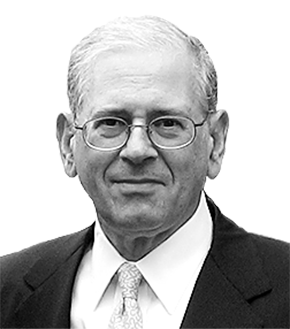
\includegraphics[width=0.5\textwidth]{assets/1453228634-RobertKahn-3820539574.png}};
        \end{tikzpicture}
        
		\vspace{2cm}
		
		{\Huge \textbf{La Bible du Réseaux en Licence}}
		
		\vspace{1cm}
		
		{\Large \textbf{Despoullains Romain}}
		
		\vfill
		
		{\Large 2023-2024}
		
	\end{center}
\end{titlepage}

\tableofcontents
\pagebreak

\section{Introduction au monde TCP‐IP}

\subsection{Introduction}

\subsection{Glossaire pour le réseau}

\subsection{Concepts de l’interconnexion}

\section{Binaire et Héxadécimal}


\subsection{Binaire}


\subsection{Puissances de 2}


\subsection{Conversions entre décimal et binaire}

\subsection{Héxadécimal}


\subsection{Puissances de 16}


\subsection{Conversions entre décimal et héxadécimal}


\subsection{Conversions entre binaire et héxadécimal}


\subsection{Binaire utile en réseau}


\subsection{Héxadécimal utile en réseau}


\section{Adressage IPV4}

\subsection{L’adressage Internet}

\subsection{Les classes d'adressage}

\section{Le protocole ARP}

\subsection{ARP}

\subsection{RARP}

\section{Le protocole IPV4}

\subsection{IPV4}

\subsection{Le datagramme IPV4}

\subsection{MTU}

\subsection{Routage des datagrammes}

\subsection{Le sous‐adressage}

\subsection{Le sous‐adressage cheatsheet}

\subsection{Le sous‐adressage variable}

\subsection{VLSM : agrégation de routes}

\section{Ethernet}

\subsection{La trame Ethernet}

\section{Le protocole UDP}

\subsection{User Datagram Protocol}

\subsection{Les ports}

\subsection{Format des messages}

\subsection{Pseudo en-tête}

\subsection{Multiplexage}

\subsection{Les ports standards}


\section{Le protocole ICMP}


\subsection{Internet Control Message Protocol}

\subsection{Format des messages}

\subsection{Format des commandes}

\subsection{Les commandes}

\subsection{Les messages d’erreur}

\subsection{Contrôle de congestion}

\subsection{Modification de route}

\subsection{Autres compte-rendus}

\section{Le protocole TCP}

\subsection{Transmission Control Protocol}

\subsection{La connexion}


\subsection{La Segmentation}


\subsection{L’Acquittement}


\subsection{Le fenêtrage}


\subsection{Gestion de la fenêtre}


\subsection{Structure du Segment}


\subsection{Format du segment}

\subsection{Mécanisme d’acquittement}


\subsection{Exemple}


\subsection{Mécanismes de retransmission}


\subsection{Gestion de la congestion}


\subsection{Mécanisme de connexion}


\subsection{Mécanisme de déconnexion}



\subsection{Ports standards}


\section{DNS}


\subsection{Domain Name System}


\subsection{La nécessité de nommer}


\subsection{Le principe pour l’utilisateur}


\subsection{L’envers du décor}


\subsection{Un système efficace}


\subsection{Les outils pour le DNS (ping -a, Nslookup, ipconfig /displaydns /flushdns}


\subsection{L’espace des noms de domaine}


\subsection{Les domaines}


\subsection{Les domaines de niveau supérieur}


\subsection{Le choix d’un nom de domaine}


\subsection{Lecture des noms}


\subsection{Les serveurs de noms}


\subsection{La délégation de zones}


\subsection{Types de serveurs de noms}


\subsection{Les résolveurs}


\subsection{Résoudre un nom}


\subsection{Les DNS Root servers}


\subsection{La résolution inverse}


\subsection{In-addr-arpa}


\subsection{Les enregistrements des DNS}


\subsection{Les logiciels DNS}


\subsection{Pourquoi installer un DNS}


\subsection{C’est quoi un nom de domaine ?}


\subsection{Domain Name Service}


\subsection{Domain Name Server}


\subsection{Serveur DNS sous Fedora (fichier hosts...)}


\subsection{Serveur DNS sous Fedora (configuration)}





\section{TCP/IP - Le routage dynamique}

\section{Le protocole IPV6}

\section{Adressage IPV6}

\section{WIFI (IEEE 802.11)}


\end{document}
